\documentclass{article}

\usepackage{graphicx}
\usepackage{tikz}
\usepackage{tikzsymbols}
\usetikzlibrary{calc,patterns,shapes.geometric}
\pagestyle{empty}
\usepackage[margin=0pt]{geometry}
\geometry{papersize={14in,12in}}

\def\centerarc[#1](#2)(#3:#4:#5){\draw[#1] ($(#2)+({#5*cos(#3)},{#5*sin(#3)})$) arc (#3:#4:#5);}

\begin{document}
	\begin{figure}
		\centering
		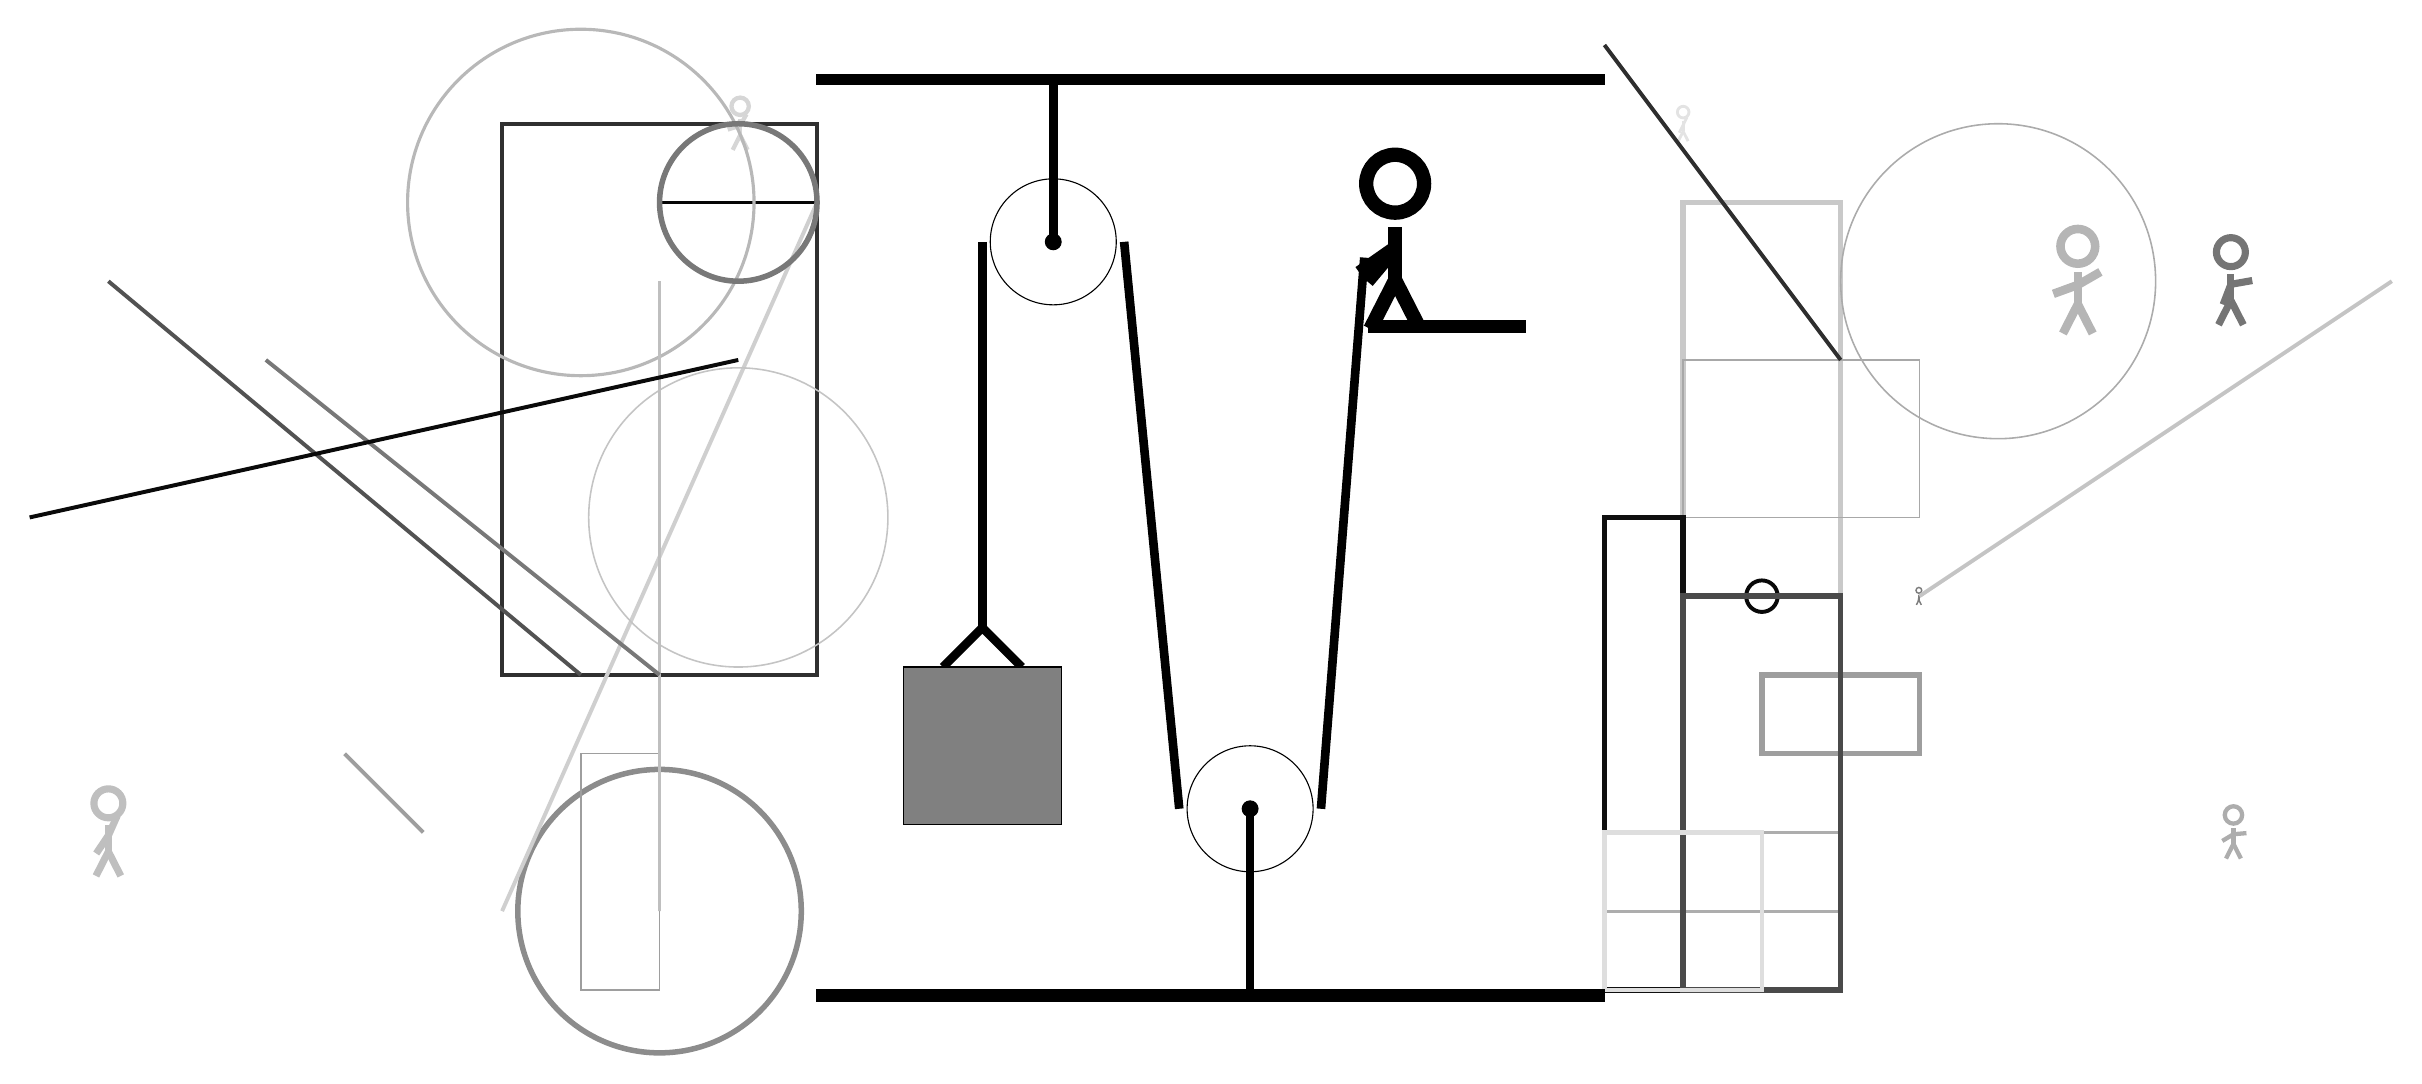
\begin{tikzpicture}
			%%%%% START %%%%%
			
			\draw[fill=black] (-2, 11.5) rectangle (8, 11.625);
			
			\draw (3.5, 2.3) circle (0.8);
			\draw[fill=black] (3.5, 2.3) circle (0.1);
			\draw[line width=1.1mm] (3.5, 2.3) -- (3.5, 0);
			
			\draw[line width=0.4mm, color=black!98] (-4, 10) rectangle (-2, 10);
			
			\draw [line width=0.7mm, color=black!45](-4, 1) circle (1.8);
			\node[line width=0.4mm, color=black!16] at (-3, 11) {\Strichmaxerl[3][18][61]};
			\draw [line width=0.5mm, color=black!97](10, 5) circle (0.2);
			\node[line width=0.4mm, color=black!25] at (-11, 2) {\Strichmaxerl[5][56][66]};
			\draw[line width=0.5mm, color=black!81] (-2, 11) rectangle (-6, 4);
			\draw[line width=0.7mm, color=black!21] (9, 5) rectangle (11, 10);
			\draw[line width=0.2mm, color=black!34] (9, 6) rectangle (12, 8);
			\draw[line width=0.5mm, color=black!19](-6, 1) -- (-2, 10);
			\draw [line width=0.4mm, color=black!28](-5, 10) circle (2.2);
			\draw[line width=0.7mm, color=black!38] (10, 4) rectangle (12, 3);
			\node[line width=0.3mm, color=black!51] at (12, 5) {\Strichmaxerl[1][82][24]};
			\node[line width=0.7mm, color=black!54] at (16, 9) {\Strichmaxerl[5][69][10]};
			
			\draw [line width=0.2mm, color=black!33](13, 9) circle (2.0);
			\draw[line width=0.2mm, color=black!38] (-4, 3) rectangle (-5, 0);
			\draw[line width=0.5mm, color=black!38](-7, 2) -- (-8, 3);
			
			\node[line width=0.4mm, color=black!29] at (14, 9) {\Strichmaxerl[6][20][30]};
			\draw [line width=0.2mm, color=black!23](-3, 6) circle (1.9);
			\draw[line width=0.7mm, color=black!94] (8, 6) rectangle (9, 0);
			\draw[line width=0.3mm, color=black!25] (-4, 1) rectangle (-4, 9);
			\node[line width=0.3mm, color=black!32] at (16, 2) {\Strichmaxerl[3][31][5]};
			\draw[line width=0.5mm, color=black!53](-4, 4) -- (-9, 8);
			
			\draw [line width=0.7mm, color=black!53](-3, 10) circle (1.0);
			\node[line width=0.3mm, color=black!11] at (9, 11) {\Strichmaxerl[2][63][64]};
			\draw[line width=0.4mm, color=black!32] (8, 2) rectangle (11, 1);
			\draw[line width=0.7mm, color=black!71] (9, 0) rectangle (11, 5);
			\draw[line width=0.5mm, color=black!23](12, 5) -- (18, 9);
			\draw[line width=0.6mm, color=black!13] (8, 0) rectangle (10, 2);
			
			\draw[line width=0.5mm, color=black!68](-5, 4) -- (-11, 9);
			\draw[line width=0.5mm, color=black!82](11, 8) -- (8, 12);
			\draw[line width=0.5mm, color=black!96](-3, 8) -- (-12, 6);
			
			\draw (1, 9.5) circle (0.8);
			\draw[fill=black] (1, 9.5) circle (0.1);
			\draw[line width=1.1mm] (1, 11.5) -- (1, 9.5);
			
			\draw[line width=1.1mm](-0.4, 4.1) --  (0.1, 4.6) -- (0.6, 4.1);
			\draw[fill=black!50] (-0.9, 4.1) rectangle (1.1, 2.1);
			
			\draw[line width=1.1mm](0.1, 9.5) -- (0.1, 4.6);
			\centerarc[line width=1.1mm](1, 9.5)(180:0:0.9)
			\draw[line width=1.1mm](1.9, 9.5) -- (2.6, 2.3);
			\centerarc[line width=1.1mm](3.5, 2.3)(180:360:0.9)
			\draw[line width=1.1mm](4.4, 2.3) -- (4.95, 9.3);
			
			\node at (5.3, 9.5) {\Strichmaxerl[10][35][-130]};
			\draw[fill=black] (5, 8.5) rectangle (7, 8.35);
			
			\draw[fill=black] (-2, 0) rectangle (8, -0.15);
			
			%%%%% END %%%%%
		\end{tikzpicture}
	\end{figure}	
\end{document}